%Empieza configuracion de capitulo
\setstretch{1.0}
\titleformat{\chapter}[block]{\Large\bfseries}{CAP'ITULO \Huge\thechapter\vspace{25 pt}}{0 pt}{\\\fontsize{26}{36}\selectfont}
\titlespacing{\chapter}{0 pt}{30 pt}{50 pt}[0 pt]
\titleformat{\section}{\Large\bfseries}{\thesection}{0 pt}{\hspace{30 pt}}
\titleformat{\subsection}{\large\bfseries}{\thesubsection}{0 pt}{\hspace{30 pt}}
\pagestyle{fancy}
\fancyhead[LO,LE]{\footnotesize\emph{\leftmark}}
\fancyhead[RO,RE]{\thepage}
\fancyfoot[CO,CE]{}
%Termina configuracion de capitulo

\chapter{Reglas de Presentaci'on} %Cambia al nombre de tu capitulo
\setstretch{1.5} %Regresa el interlineado a 1.5

\normalsize
\noindent
Este manual de tesis se basa, en parte, del estilo establecido por la Rector'ia de la Universidad Virtual (UV) del Sistema Tecnol'ogico de Monterrey \cite{Demo:manualUV} y publicado por la American Psychological Association (APA) \cite{Demo:APA,Demo:manualAPA}. Los alumnos de las maestr'ias de la EGIA (Escuela de Graduados en Ingenier'ia y Arquitectura) del ITESM Campus Guadalajara deben considerar que es imprescindible apegarse a las reglas de estilo que se presentan en este manual.

Las siguientes reglas de formato son aplicables a las maestr'ias ofrecidas por la EGIA. Aseg'urate de seguirlas minuciosamente. Este manual est'a escrito estrictamente de acuerdo a las reglas generales y particulares que se mencionan a continuaci'on, as'i que le sirve como modelo para escribir tanto su documento de anteproyecto de tesis, como su documento final.

\section{Reglas generales}
\noindent
\begin{enumerate}
	\item Imprime solamente en un lado de la p'agina.
	\item Usa sangr'ias para cada p'arrafo nuevo, a excepci'on del primer p'arrafo que sigue a un cap'itulo, secci'on o subsecci'on.
	\item Inicia cada cap'itulo en una p'agina nueva.
	\item No dejes l'ineas aisladas al inicio de una p'agina. Escribe por lo menos un p'arrafo en su parte superior de al menos cuatro l'ineas.
	\item Utilizar una p'agina nueva para las referencias bibliogr'aficas como se muestra en este manual.
	\item Separa las s'ilabas siguiendo estrictamente las reglas gramaticales.
	\item Los trabajos producidos en impresoras de puntos son inaceptables, as'i como aqu'ellos producidos en otros medios que no aseguren una alta calidad de impresi'on. Se recomienda utilizar impresoras del tipo postscript.
	\item Centra los t'itulos de las p'aginas preliminares y la bibliograf'ia. Por ejemplo: Dedicatoria, Agradecimientos, Resumen, Contenido, Lista de Tablas y figuras y Bibliograf'ia (ver como ejemplo las p'aginas preliminares de este manual).
	\item Los cap'itulos del cuerpo del documento deben estar justificados a la izquierda y escritas en negritas. El t'itulo del cap'itulo correspondiente lleva may'usculas al inicio de todas las palabras, a excepci'on de las palabras cortas como: de, un, una, el, la, etc. Por ejemplo: \textbf{Dise'no de una Plataforma de Decodificaci'on}.
	\item Las subdivisiones de los cap'itulos deben estar escritas en negritas y min'usculas a excepci'on de la primera letra de la oraci'on.
	\item La silustraciones y tablas podr'an ser presentadas horizontalmente si no caben de manera vertical.
\end{enumerate}

\section{Tipo de letra}
\noindent
\begin{enumerate}
	\item Si emplea el procesador de textos Word\copyright  de Microsoft\textsuperscript{\texttrademark} o alguno similar, utilice letra de tipo Times New Roman de tama'no 12 puntos para la redacci'on del documento. Si usted escribe el documento en \LaTeX, utilice el layout disponible para tal efecto. No use letra cursiva excepto para las palabras cuyo origen sea de un idioma diferente al Espa'nol.
	\item Usa el mismo tipo de letra para todo el manuscrito; incluyendo las p'aginas preliminares, las referencias bibliogr'aficas y los anexos.
	\item Podr'as usar tama'nos reducidos de letras solamente en los pies de p'agina, pies de ilustraciones y tablas y citas textuales de otros trabajos.
	\item Usa el mismo tipo de letra para numerar ilustraciones y tablas, el cual puede ser diferente del tipo de letra usado para el texto del trabajo\footnote{De preferencia utilizar todas las especificaciones de este manual. En caso de utilizar, por ejemplo, el editor de texto Word ajustar las caracter'isticas del mismo para que cumplan con todas las especificaciones.\label{footnote}}.
	\item Usa numeraci'on ar'abiga (1, 2, 3, etc.) en la numeraci'on de secciones, subsecciones y en los n'umeros de p'agina. No se permiten cursivas para estos n'umeros.
\end{enumerate}

\section{Ecuaciones}
\noindent
\begin{enumerate}
	\item La presentaci'on de las ecuaciones deber'a realizarse con el uso de un editor de ecuaciones.
	\item Puedes utilizar un estilo de letra diferente al del texto para las ecuaciones.
	\item Puedes numerar las ecuaciones a trav'es del escrito si lo consideras pertinente. Si es as'i, poner la numeraci'on justificada a la derecha de las ecuaciones. Ejemplo:
\end{enumerate}

Si consideramos una transmisi'on de s'imbolos sobre un canal con modulaci'on BPSK (\emph{Binary Phase Shift Keying}) no codificada, y utilizamos una demodulaci'on coherente\footnote{El demodulador conoce la frecuencia y la fase de la onda recibida.\label{footnote}}, la probabilidad de error \begin{math}P_b(e)\end{math} sobre un canal gaussiano se puede expresar bajo la forma [7]:
\[P_b(e)=Q\left(\sqrt{\frac{2E_b}{N_0}}\right)\]
donde \begin{math}Q(.)\end{math} es la funci'on de error de una variable aleatoria gaussiana normalizada:
\[Q(x)=\int_x^\infty \frac{1}{\sqrt{2\pi}}e^{-\frac{u^2}{2}}du\]
El l'imite de la capacidad de informaci'on cuando \begin{math}R \to 0\end{math} es derivado de la ecuaci'on \begin{math}\lim_{R \to 0} [1-H_b(e)]=\frac{E_b}{(ln 2) N_0}\end{math}. Re-escribi'endolo, obtenemos:
\[
\begin{aligned}
\frac{E_b}{N_0}&=ln 2(1-H_b(e))\\
&=ln 2(1+P_b(e)log_2P_b(e)+(1-P_b(e))log_2(1-P_b(e)))
\end{aligned}
\]

\section{Figuras}
\noindent
En esta secci'on se muestran algunos ejemplos de figuras, ilustraciones y gr'aficas extra'idas de la referencia \cite{Demo:phdTesis} que pueden servir de modelo en la redacci'on del documento de tesis.
\begin{figure}[H]
\centering
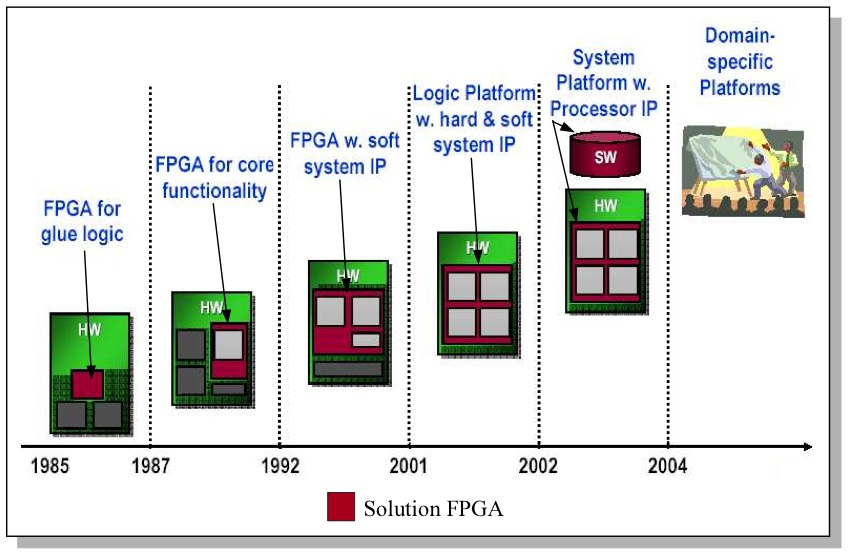
\includegraphics[width=0.75\textwidth]{images/figura4_1}
\caption{Evoluci'on de los FPGA hacia soluciones completas en un solo chip.}
\label{fig:4.1}
\end{figure}

\begin{figure}[H]
\centering
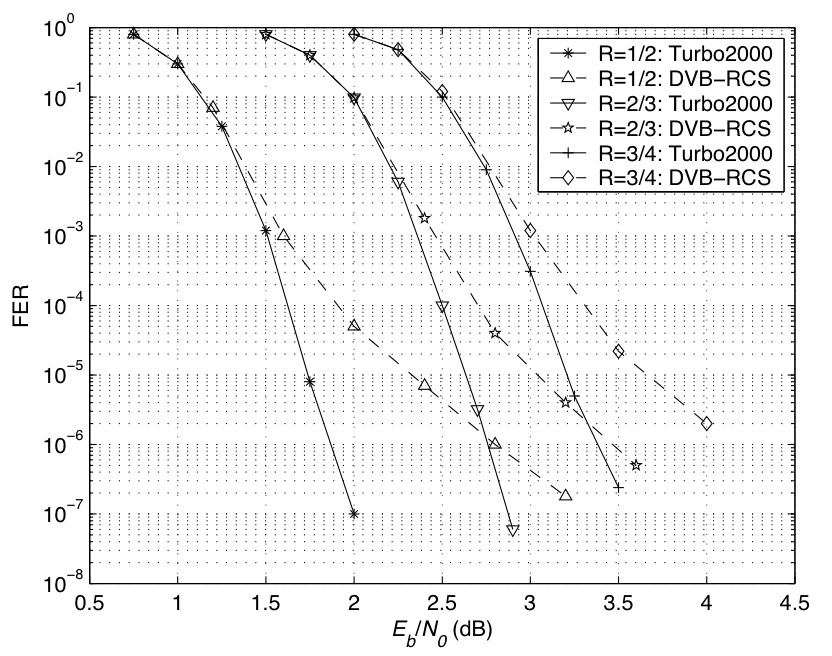
\includegraphics[width=0.7\textwidth]{images/figura4_2}
\caption{Comparaci'on del desempe'no de FER entre Turbo2000 y DVB-RCS. Par'ametros de la simulaci'on: Tama'no = 188 bytes, 8 iteraciones, q=4, QPSK y AWGN.}
\label{fig:4.2}
\end{figure}

\begin{figure}[H]
\centering
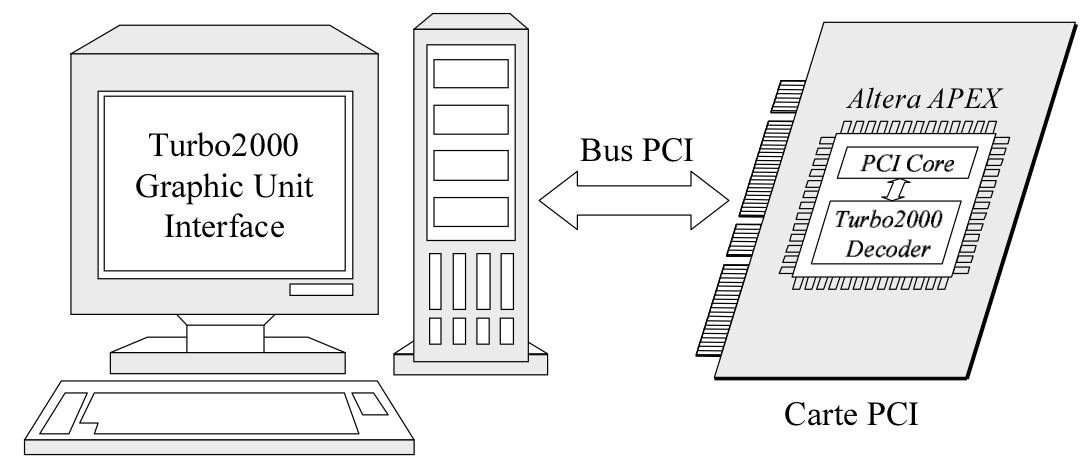
\includegraphics[width=0.9\textwidth]{images/figura4_3}
\caption{Plataforma Turbo2000.}
\label{fig:4.3}
\end{figure}

\section{Tablas}
\noindent
Esta secci'on presenta algunos ejemplos de formatos de tablas extra'idas de la referencia \cite{Demo:phdTesis} que se pueden usar en el documento de tesis.
\begin{table}[H]
	\begin{center}
		\begin{tabular}{ | c | c | c | }
			\hline
			& & \\[-18pt]
			\emph{q} bits	&	\emph{L}\subscript{max}	&	\begin{math}\Delta\end{math}\subscript{max} \\[3pt]
			\hline \hline
			& & \\[-18pt]
			2 & 11 & 8 \\[8pt]
			3 & 33 & 24 \\[8pt]
			4 & 77 & 82 \\[8pt]
			5 & 165 & 123 \\[8pt]
			6 & 341 & 395 \\[5pt]
			\hline
		\end{tabular}
	\end{center}
	\caption{Din'amica de m'etricas para diferentes valores de q con $R =1/2, E_b/N_0 = 2 dB$ y modulaci'on QPSK.}
\end{table}

\begin{table}[H]
	\begin{center}
	\begin{threeparttable}
	\begin{tabular}{ | c || c | c | }
		\hline
		& & \\[-8pt]
		Unit'e	&	\# Add./Soustr.	&	\# min(.)	\\[3pt]
		\hline \hline
		& & \\[-18pt]CMB			&	22					&	0					\\& & \\[-18pt]\hline
		& & \\[-18pt]Proc. ACS		&	$2^m \cdot N_a = 64$	&	$N_s \cdot (2^m-1)=48$	\\& & \\[-18pt]\hline
		& & \\[-18pt]CP			&	$2^m \cdot N_a = 64$	&	$2^m \cdot (N_s-1)=60$	\\& & \\[-18pt]\hline
		& & \\[-18pt]CIE\tnote{a}	&	$2^{m+1} = 8$		&	$2^m-1=3$			\\& & \\[-18pt]\hline
		& & \\[-18pt]CCD\tnote{b}	&	1					&	2					\\& & \\[-18pt]\hline
		& & \\[-18pt]CCA\tnote{b}	&	1					&	2					\\
		\hline
	\end{tabular}
	\setstretch{1.0}
	\begin{tablenotes}
		\item[\tiny a]{\tiny No se consideran los sub-bloques de actualizaci'on de los datos extr'insecos.}
		\item[\tiny b]{\tiny El comparador de salida es considerado como un sumador.}
	\end{tablenotes}
	\setstretch{1.5}
	\end{threeparttable}
	\end{center}
	\caption{Complejidad de c'alculo de las unidades del decodificador Turbo2000.}
\end{table}

\begin{table}[H]
	\begin{center}
	\begin{threeparttable}
	\begin{tabular}{ | l || l | l | l |}
		\hline
		& & & \\[-18pt]
		\textbf{Tratamiento}		&	\textbf{Unidades activas}		&	\textbf{\# Add./Soustr.}	&	\textbf{\# min(.)}	\\[3pt]
		\hline \hline
		& & &\\[-18pt]RETOUR 2	&	CMB, Proc. ACS \emph{Retour}&	$22+2^m \cdot N_s$			& $N_s \cdot (2^m-1)$\\& & &\\[-18pt]
		& & &\\[-18pt]			&						&	86						& 48\\& & &\\[-18pt]\hline
		& & &\\[-18pt]ALLER 2		&	CMB, Proc. ACS \emph{Aller},&	$22+2^{m+1} \cdot (N_s+1)$	& $N_s \cdot (2^m-1)-1$\\& & &\\[-18pt]
		& & &\\[-18pt]			&	CP, CIE				&	158						& 111\\& & &\\[-18pt]\hline
		& & &\\[-18pt]RETOUR 1	&	CMB, Proc. ACS \emph{Retour}&	$22+2^m \cdot N_s$			& $N_s \cdot (2^m-1)$\\& & &\\[-18pt]
		& & &\\[-18pt]			&						&	86						& 48\\& & &\\[-18pt]\hline
		& & &\\[-18pt]ALLER 1		&	CMB, Proc. ACS \emph{Aller},&	$24+2^{m+1} \cdot (N_s+1)$	& $N_s \cdot (2^m-1)+3$\\& & &\\[-18pt]
		& & &\\[-18pt]			&	CP, CIE, CDD, CCA			&	160						& 115\\[3pt]
		\hline
	\end{tabular}
	\end{threeparttable}
	\end{center}
	\caption{Complejidad de c'alculo seg'un el tratamiento del decodificador Turbo2000.}
\end{table}

\section{M'argenes}
\noindent
\begin{enumerate}
	\item El margen izquierdo (del lado del encuadernado) ser'a de tres cent'imetros, incluyendo tablas e ilustraciones. El margen derecho ser'a de dos cent'imetros.
	\item Los m'argenes superior e inferior ser'an de dos cent'imetros. Esto no incluye los encabezados o pies de p'agina.
	\item Las p'aginas horizontales deber'an tener en la parte superior de la hoja un margen de tres cent'imetros; para que, al ubicarlas de manera vertical en el manuscrito, este margen coincida con el requerido para el encuadernado.
\end{enumerate}

\section{Espacios}
\noindent
\begin{enumerate}
	\item El texto del trabajo se har'a a doble espacio como viene en este manual.
	\item Se permite usar espacio sencillo en el 'indice de contenido, de ilustraciones, de tablas y en los ap'endices.
	\item El espacio sencillo es obligatorio para citas textuales en p'arrafos de otros autores, pies de figura, pies de tabla y pies de p'agina. Ejemplo de una cita textual \cite{Demo:phdTesis}:\\
	
	\setstretch{1.0}
	\small
	``Un turbo-c'odigo m-binario est'a compuesto de dos c'odigos CRSC m-binarios id'enticos concatenados en paralelo a trav'es de un permutador. La t'ecnica de terminaci'on circular es utilizada en estos c'odigos bidimensionales para codificar bloques sin hacer uso de bits de terminaci'on. La tasa de codificaci'on global R para un turbo-c'odigo es igual a m/(m + 2).''
\end{enumerate}
\setstretch{1.5}

\section{P'aginas}
\noindent
\begin{enumerate}
	\item Se numeran todas las p'aginas a partir de las p'aginas de Dedicatoria, Agradecimientos, Resumen, Contenido, Lista de Tablas y Figuras, Bibliograf'ia, Ap'endices y Vitae.
	\item No se numeran las p'aginas de la Portada y de Firmas.
	\item Coloca los n'umeros de p'aginas en el centro del margen inferior al inicio de un cap'itulo, y en el margen superior derecho para las dem'as. Las p'aginas en las que aparecen cuadros y gr'aficas tambi'en deben numerarse y su disposici'on (vertical u horizontal) no debe alterar la posici'on del n'umero de p'agina.
	\item Las p'aginas que incluyen la Dedicatoria, Agradecimientos, Resumen, Contenido, Lista de Tablas y Figuras utilizan la numeraci'on romana, es decir, I, II, III, IV, etc.
	\item Las p'aginas a partir del cap'itulo 1 utilizan la numeraci'on ar'abiga, es decir, 1, 2, 3, etc. Esto considera tambi'en a la Bibliograf'ia, los Ap'endices y el Vitae.
	\item No uses la palabra ``p'agina'' antes de la numeraci'on de las p'aginas.
	\item Usa el mismo tipo de letra para todos los n'umeros de p'agina.
\end{enumerate}

\section{Manuscrito final del documento de tesis}
\noindent
El manuscrito final de tesis deber'a respetar el siguiente orden:
\begin{enumerate}
	\item Portada del empastado (obligatoria): No se coloca el n'umero de p'agina y no se cuenta. Ver primera p'agina del manual.
	\item P'agina de Firmas (obligatoria): No se coloca el n'umero de p'agina y no se cuenta. Ver segunda p'agina del manual.
	\item Dedicatoria (opcional): Se coloca p'agina con n'umero romano en min'uscula.
	\item Ep'igrafe (opcional): Se coloca p'agina con n'umero romano en min'uscula.
	\item P'agina de reconocimientos o agradecimientos (opcional): Se coloca p'agina con n'umero romano en min'uscula.
	\item Resumen (obligatorio): Se coloca p'agina con n'umero romano en min'uscula.
	\item 'Indice de contenido (obligatorio): Se coloca p'agina con n'umero romano en min'uscula.
	\item Lista de tablas (puede ser requerido): Se coloca p'agina con n'umero romano en min'uscula.
	\item Lista de ilustraciones o gr'aficas (puede ser requerido): Se coloca p'agina con n'umero romano en min'uscula.
	\item Lista de abreviaturas (opcional): Se coloca p'agina con n'umero romano en min'uscula.
	\item Glosario (opcional): Se coloca p'agina con n'umero romano en min'uscula.
	\item Introducci'on (obligatoria). La introducci'on ser'a considerada como el primer cap'itulo del cuerpo del manuscrito. A partir de aqu'i inicia la paginaci'on ar'abiga.
	\item Cuerpo del manuscrito (obligatorio): Continu'a la paginaci'on ar'abiga.
	\newpage
	\item Referencias bibliogr'aficas (obligatorio): Continu'a la paginaci'on ar'abiga. Utilizar el formato del IEEE como viene en la siguiente p'agina.
	\item Ap'endices (opcional): Continu'a la paginaci'on ar'abiga.
	\item Vitae (obligatorio): Continu'a la paginaci'on ar'abiga.
\end{enumerate}

\clearpage